%%%%%%%%%%%%%%%%%%%%%%%%%%%%%%%%%%%%%%%%%
% ELEE	3720 Electromechanical Energy Conversion: Report template
% By Ratheesh Ravindran
%%%%%%%%%%%%%%%%%%%%%%%%%%%%%%%%%%%%%%%%%
\documentclass[12pt]{article}
\usepackage{setspace}
\usepackage[english]{babel}
\usepackage[utf8x]{inputenc}
\usepackage{amsmath}
\usepackage{graphicx}
\usepackage[procnames]{listings}
\graphicspath{{Images/}}
\usepackage[colorinlistoftodos]{todonotes}
\usepackage{hyperref}
\usepackage{floatrow}
%\usepackage{fancyhdr}
%\pagestyle{fancy}

\begin{document}
\definecolor{keywords}{RGB}{255,0,90}
\definecolor{comments}{RGB}{0,0,113}
\definecolor{red}{RGB}{160,0,0}
\definecolor{green}{RGB}{0,150,0}
 
\lstset{language=Python, 
        basicstyle=\ttfamily\small, 
        keywordstyle=\color{keywords},
        commentstyle=\color{comments},
        stringstyle=\color{red},
        showstringspaces=false,
        identifierstyle=\color{green},
        procnamekeys={def,class}}
 
\begin{titlepage}
\newcommand{\HRule}{\rule{\linewidth}{0.1mm}} 
\center % Center everything on the page
 
%---------------------------------------------------------------------------------
%	HEADING SECTIONS (Enter the Homework/assignment No., only)
%---------------------------------------------------------------------------------
\textsc{\Large Middle East Technical University}\\[0.5cm] % heading course Number
\textsc{\Large Department of Computer Engineering}\\[0.5cm] % heading course name
%\textsc{\large Homework/Assignment No:- }\\[0.5cm] % Minor heading
%---------------------------------------------------------------------------------
%	TITLE SECTION (Replace 'TITLE' with the Homework/assignment Name/title)
%---------------------------------------------------------------------------------

\HRule \\[0.4cm]
{ \huge CENG300}\\[0.3cm]
{ \huge SUMMER PRACTICE REPORT}\\[0.1cm] % Title of your Homework/assignment
%\HRule \\[1.5cm]
 
 \textsc{JotForm Yazılım A.Ş.}\\[0.1cm]
 \textsc{Hacettepe Teknokent Safir Bloklar C Blok Kat:6}
 \HRule \\[1.5cm]
 
%---------------------------------------------------------------------------------
%	AUTHOR SECTION (EDIT THE NAME and T.NO., only)
%---------------------------------------------------------------------------------

\begin{minipage}{0.4\textwidth}
\begin{flushleft} \large

\emph{Student's Name:}\\
Ozan \textsc{Şan}\\  % Enter Your name and T.No.
\end{flushleft}
%\begin{flushleft} \large

%\emph{Author 2:}\\
%Amna \textsc{Author-2}\\ T.No.  % Enter Your name and T.No.
%\end{flushleft}


\end{minipage}
\begin{minipage}{0.4\textwidth}
\begin{flushright} \large
\emph{Instructor:} \\
Prof.Dr.Göktürk Üçoluk% \textsc{Üçoluk} % Supervisor's Name
\end{flushright}
\end{minipage}\\[1cm]
{\large \today}\\[1cm] % Date, change the \today to a set date if you want to be precise

\includegraphics{cmetusmallest.png}\\[1.0cm]% \\[0.5cm] % 
%\vfill % Fill the rest of the page with white-space
Start Date: 10.06.2019 \\
End Date: 22.07.2019 \\
Total Working Days: 30 \\[1.2cm]
Student's Signature \hspace{150px} Organization Approval \\
\end{titlepage}
%%
% GradingRubric.tex
% This page will be the 2nd page of your report and will be used for grading the homework/assignment.
\section*{Grading Rubric - Information to Students}

Grading rubric that will broadly apply to assessing performance. That is, assessment exercises that are associated with a predominantly qualitative rather than quantitative character. If, for a particular exercise, there is substantial deviation from the scheme outlined below, I will let you know! Note: Be aware that if your “Quality of Presentation” is poor, it could impact scores assigned for the other two categories! (DO NOT EDIT THIS PAGE)
%\hspace*{-1.5in}
\begin{figure}[ht!]
    \centering
    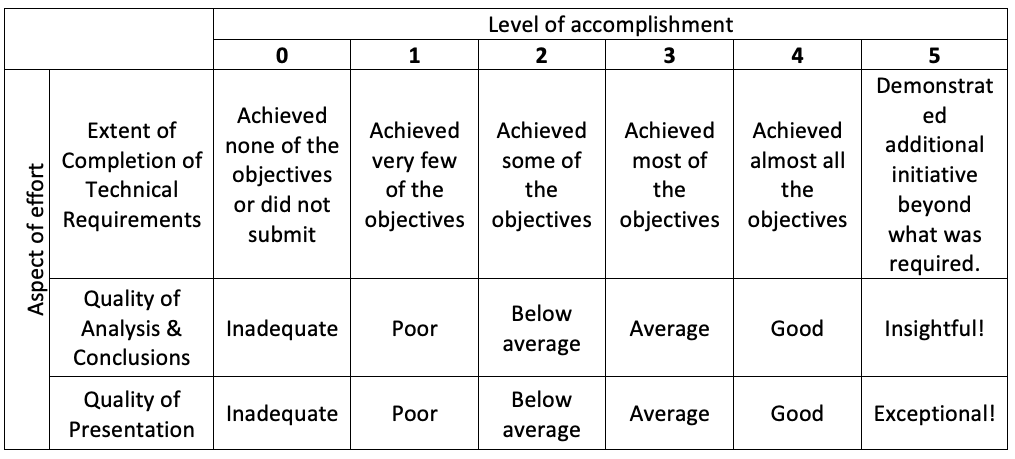
\includegraphics[scale=0.450]{LevelOfAccomplishments.png}
    \caption{Level of accomplishments}
    \label{fig:Level of accomplishments}
\end{figure}
\begin{table}[h]
    \centering
    \begin{tabular}{|c|c|}
    \hline
        Level &  Score \\
        \hline
        \hline
        5 &  12 (bonus!) \\
        \hline
        4: (`A`) &  10 \\
        \hline
        3: (`B`) &  8 \\
        \hline
        2: (`C`) &  6 \\
        \hline
        1: (`D`) &  4 \\
        \hline
        0: (`F`) &  0-2 \\
        \hline
    \end{tabular}
    \caption{Mapping of “Level” to “Score”}
    \label{tab:Mapping}
\end{table}
\begin{itemize}
    \item \textbf{Student's Level/Score (To be entered by Professor/GTA):}
\end{itemize}



\tableofcontents          % Required
%\listoffigures
%\listoftables
\newpage

% Do not edit the below sections, enter all details in respective chapters
% Add the images/screen-shorts to the image folder and insert them in the respective chapters

\section{Introduction}

% Introduction

I have completed my internship at JotForm Yazılım A.Ş., R\&D office, at Hacettepe Teknokent, Ankara. \\
My internship was about Time Series Analysis (TSA), and an implementation of a prediction system,
using metrics provided by JotForm. The metrics are numerical, and represents the state (mainly, financial state)
of the company. Using SARIMAX modelling, I have made a system which makes predictions about the future,
and, when in need, can be exported as a graph, and be further evaluated by the Data Science team of JotForm. This
will be further explained in further sections of this document.




\section{Project}
The project I have completed is called JFM Overseer. Overseer is an application written in Python 3.7, and is capable of predicting time series. Below is a screenshot taken from the application: \\
\begin{center}


\begin{figure}[th!]
    \centering
    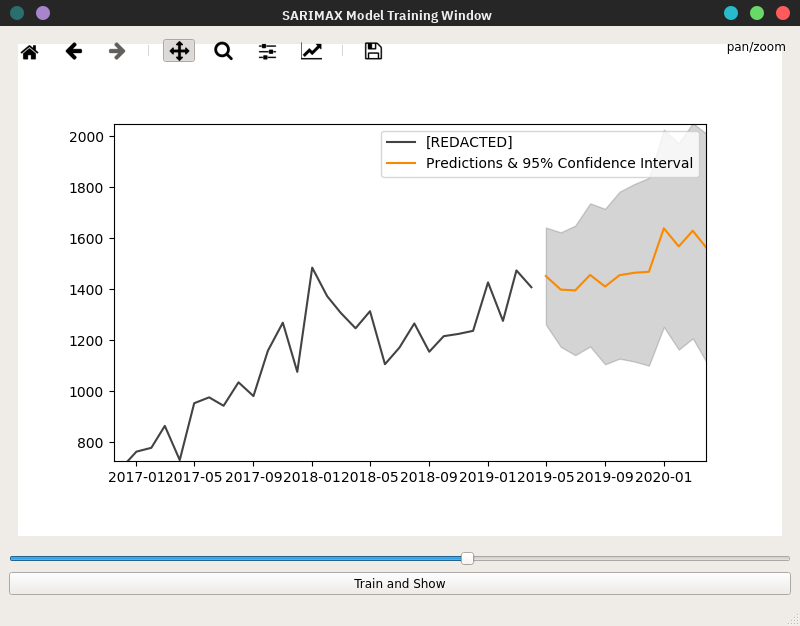
\includegraphics[width=0.6\textwidth]{Images/sarimax-window.png}
    \caption{A Screenshot From The Application}
    \label{fig:SARIMAXWindow}
\end{figure}
\end{center}
The components and how to set them up are explained in Section \ref{sec:pyqt5}.
\subsection{Analysis Phase}
Analyzing the problem of efficiently forecasting time series was especially difficult because the texts for this problem is intended for statisticians and economists, but as a future computer engineer, I've found that practical examples on \textbf{Kaggle} and other Data Science learning sites were especially helpful. 
\subsection{Design Phase}
The overall structure of the application is as in the following diagram:\\
\begin{table}[ht!]
\centering
\begin{tabular}{|l|ll} 
\cline{1-1}\cline{3-3}
GUI components (PyQT5) & \multicolumn{1}{l|}{$\rightarrow$} & \multicolumn{1}{l|}{Matplotlib}  \\ 
\cline{1-1}\cline{3-3}
Facebook Prophet \& StatsModels  &                         &                        \\ 
\cline{1-1}
Pandas  &                         &                        \\ 
\cline{1-1}
Time Series Data (.csv)  &                         &                        \\
\cline{1-1}
\end{tabular}
\end{table} \\
In Section \ref{sec:pyqt5} the visual design phase is explained further.

\subsection{Implementation Phase}
This is quite a lengthy topic, and it will be discussed further, beginning with Section \ref{sec:tsds} and until Section \ref{sec:testing}.
\subsection{Time Series Data Specifications}
\label{sec:tsds}
Overseer is a tool to analyze Time Series data, which must be given to the program as .csv files, with the following structure: \\

\begin{table}[ht]
\centering
\begin{tabular}{| l | l |}
$t$    & $y$    \\
$t_0$  & $y_0$  \\
\vdots & \vdots
\end{tabular}
\end{table}
In this representation, $t$ must correspond to a date-time value, mainly, parse-able by Matplotlib and other software used. The values for y must be integers. \\
This lets us create a function $F(t) = y$, which is useful in upcoming definitions.
My goal was mainly to produce a prediction, namely, we have to define values $m_t, n_t$ such that for any $t > t_{end}$, where the last observed point of the function F is at time $t_0 + end$, the equation
\begin{equation*}
	P(m_{t} < F(t) < n_{t}) = 0.95
\end{equation*}
must hold. This corresponds to creating a $95\%$ probability interval for the possible observed values of the function $F$ in the future, and means that we have made a prediction. The values $m_t$ and $n_t$ can be averaged to yield a possible future value of $F$. For making this possible, we must first structure the data in a suitable way.
\subsection{Pandas}
pandas is an open source, BSD-licensed library providing high-performance, easy-to-use data structures and data analysis tools for the Python programming language.\cite{Pandas}
\subsubsection{Installation}
Since our app runs best on Anaconda distributions, the suitable way to install pandas is:
\begin{lstlisting}[language=bash, backgroundcolor = \color{lightgray}]
conda install pandas
\end{lstlisting}
One can also use, in a plain Python environment,
\begin{lstlisting}[language=bash, backgroundcolor = \color{lightgray}]
pip install pandas
\end{lstlisting}
\subsubsection{Usage}
An example of loading a .csv file, processing it to a uniform format, namely, a ``timeseries":
\begin{lstlisting}[language=Python]
	import pandas as pd
	df = pd.read_csv(FILENAME)
	# FBProphet expects the data
	# to conform to a format, as such:
	df.columns = ['ds', 'y']
	# We need to parse the dates
	# to yield date-time objects
	df['ds'] = df['ds'].apply(pd.to_datetime)
	# After this, df is ready to be processed. 
\end{lstlisting}
If needed, multiple sources can be loaded and processed to yield a single table using Pandas, as if working with a spreadsheet editor.
\subsection{Facebook Prophet}
Prophet is a forecasting procedure implemented in R and Python. It is fast and provides completely automated forecasts that can be tuned by hand by data scientists and analysts \cite{FBProphet}. The process used in automating FBProphet was explained in \cite{ForecastingAtScale}.
\subsubsection{Installation}
For this package, and with all other packages, it is recommended to use Anaconda distributions. \\
For an Anaconda distributed Python installation, one can simply use:
\begin{lstlisting}[language=bash]
conda install -c conda-forge fbprophet
\end{lstlisting}
to install Facebook Prophet. For certain situations (for example, working in a computer with little storage space),
\begin{lstlisting}[language=bash]
pip install fbprophet
\end{lstlisting}
should still work.
\subsubsection{Usage}
The usage of FBProphet follows a simple direction, we first load and structure the data for Prophet, import fbprophet and start an instance of the class ``Prophet", fit the data and create a future dataframe for Prophet, then see the results for the future dataframe with the help of Prophet. As example:
\begin{lstlisting}[language=Python]
	# In previous sections, we have
	# already loaded the data in the
	# 'df' variable.
	import fbprophet as fbp
	prophet = fbp.Prophet()
	# We then fit the timeseries:
	prophet.fit(df)
	# We create a future dataframe
	# for seeing the results
	# We provide the periods as 12
	# for yearly seasonality
	future = prophet.make_future_dataframe(periods=12)
	# we can now see the results
	forecast = prophet.predict(future)
	# forecast variable will have
	# columns as 'yhat', 'yhat_lower',
	# and 'yhat_upper'
\end{lstlisting}
\subsubsection{Possible issues with Facebook Prophet}
\label{sec:prophet-issues}
The developers of Facebook Prophet have their own datetime format for parsing, and this causes issues. In the source code of the package, there is a line:
\begin{lstlisting}[language=Python]
pandas.plotting.deregister_matplotlib_converters()
\end{lstlisting}
This line of code breaks the system if we are including Prophet after Pandas as I've used \textbf{pd.to\_datetime} for converting strings of dates into datetime objects, and the solution in my case was adding the following line wherever I've imported Facebook Prophet:
\begin{lstlisting}[language=Python]
pandas.plotting.register_matplotlib_converters()
\end{lstlisting}
This sadly breaks the plotting functionality of Facebook Prophet, but in my case, as I've done all of my plotting with Matplotlib, it does not really matter.
\subsection{Statsmodels}
statsmodels is a Python module that provides classes and functions for the estimation of many different statistical models, as well as for conducting statistical tests, and statistical data exploration.\cite{StatsModels}
\subsubsection{Installation}
As usual, we both have a Conda way and a native Pip way of installing the package.
\begin{lstlisting}[language=bash, backgroundcolor = \color{lightgray}]
	conda install -c conda-forge statsmodels
\end{lstlisting}
\centerline{or...}
\begin{lstlisting}[language=bash, backgroundcolor = \color{lightgray}]
	pip install -U statsmodels
\end{lstlisting}
\subsubsection{Usage}
The usage for this environment is significantly more involved than of Facebook Prophet. First of all, since statsmodels offers a lot of statistical framework, it can simply not operate on the principle ``set, and go". We will use a type of modelling in Econometrics called a \textbf{SARIMAX} model, short for ``Seasonal AutoRegressive Integrated Moving Average with eXogenous regressors model". We need to determine three variables (namely, $P$, $D$ and $Q$, for each of the AutoRegressive, Moving-Average and Residual parts) for trying a SARIMAX model, and select the best one for the purpose to display on the screen. \\
Normally, this process is done by a statistics graduate, or a senior Data Scientist with a professional background, but, in our case, we have found a more adept solution for our problem. \\
For assessing a model's usability, Akaike's Information Criterion was used. The model which yields the lowest AIC score was to be used. \\
The following example code, as it is implemented in the project, uses a simple grid search to find the variables $P$, $D$ and $Q$. Itertools module facilitates an easy interface for checking all possible combinations within constraints. The following code segments represent how this step was implemented within the project:\\
\begin{lstlisting}[language=Python]
import itertools
import statsmodels.api as sm
import numpy as np
# We need to limit the computation time,
# So we are only looking on the range [0, 2].
p = d = q = range(0, 2)
# Generating all possible combinations of these variables
pdq = list(itertools.product(p, d, q))
# Seasonal data will be assumed to have the same variables
# Seasonality is set to 12, indicating months.
seasonal_pdq = [(x[0], x[1], x[2], 12) for x in pdq]
resBest = np.inf # Initially, we will assume the worst
for param in pdq:
  for param_seasonal in seasonal_pdq:
    try:
      mod = sm.tsa.statespace.SARIMAX(time_series,
                                      order=param,
                                      seasonal_order=param_seasonal,
                                      enforce_stationarity=False,
                                      enforce_invertibility=False)

      results = mod.fit()
        if results.aic < resBest:
          resBest = results.aic
          paramreality = param
          paramss = param_seasonal
     except:
       continue
\end{lstlisting}
\vspace{1.0cm}
After this -lengthy- process is completed, we can take a look at our best results, using:\\
\begin{lstlisting}[language=Python]
mod = sm.tsa.statespace.SARIMAX(endog = self.time_series,                                            
      order = self.sarimax_parameters[0],
      seasonal_order= self.sarimax_parameters[1],
      enforce_stationarity= False,
      enforce_invertibility= False)
res = mod.fit()
pred = res.get_prediction(start = pd.to_datetime(time_series.index[-1]),
      dynamic = True,
      end = END_OF_PREDICTION)
confidence_interval = pred.conf_int()
\end{lstlisting}
This typically yields similar results to Facebook Prophet's predictions, but allows for more fine tuning of the model, although it costs more time, it is recommended to run a SARIMAX model on the data even though the Prophet predictions are usable as they are.
\subsubsection{Possible Drawbacks of StatsModels}
Performing a grid search is not a computationally easy task. A quad-core CPU takes minutes until completion of a model for a range of $[0, 4]$. And because no multiple-core functionality is defined for SARIMAX models as it seems in Statsmodels, Core 0 of the machine's CPU will be loaded heavily. This can be bypassed by implementing functionality of multiple core execution, but, as this models are enough for monthly resolutions, this was not needed.
\subsection{PyQt5 (QT Framework)}
\label{sec:pyqt5}
PyQt is a set of Python v2 and v3 bindings for The Qt Company's Qt application framework and runs on all platforms supported by Qt including Windows, OS X, Linux, iOS and Android. PyQt5 supports Qt v5.\cite{PyQt}
\subsubsection{Installation}
\begin{lstlisting}[language=bash, backgroundcolor = \color{lightgray}]
	conda install PyQt5
\end{lstlisting}
\centerline{or...}
\begin{lstlisting}[language=bash, backgroundcolor = \color{lightgray}]
	pip install pyqt5
\end{lstlisting}
Appropiate Qt bindings will be located and installed as necessary.
\subsubsection{Usage}
Usage of the Qt framework is done in two different ways, one of them is coding the GUI elements in Python, and the other is using Qt Designer. For all intents and purposes, Qt Designer is much easier to use when positioning and constraining different elements on the viewport.
\begin{figure}[hbt!]
    \centering
    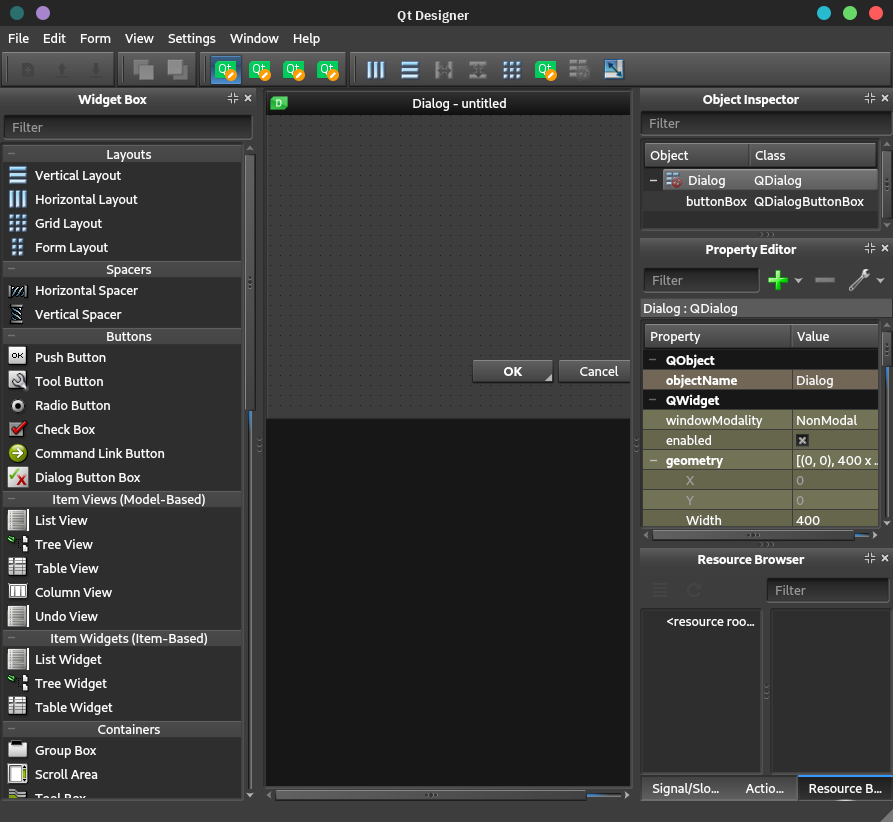
\includegraphics[width=0.9\textwidth]{Images/QtWindow.png}
    \caption{An overview of Qt Designer.}
    \label{fig:QTDesigner}
\end{figure} \\
After completing a design for a particular window, Qt Designer outputs a file with .ui extension. This can be loaded in Python to define further elements, such as relevant function calls for when certain buttons are pressed, etc. Here is an example of such an usage:
\begin{lstlisting}[language=Python]
from PyQt5.QtWidgets import *
from PyQt5.uic import loadUi
# We inherit a class, QMainWindow
# to be able to have basic functionality
# in our window.
class MatplotlibWidget(QMainWindow):
  def __init__(self):
    # Inherited class is initialized
    QMainWindow.__init__(self)
    #.ui file is loaded
    loadUi("mainWindow.ui", self)
    # Then, necessary adjustments can be made
    self.setWindowTitle("JFM Overseer")
    # for example, "pushButton_select_files" is
    # a name defined in "mainWindow.ui", and
    # QT keeps track of each button.
    self.pushButton_select_files.clicked.connect(CALLBACK)
    # This can be further examplified.
\end{lstlisting}
\subsubsection{Possible drawbacks of PyQt5}
Qt Library has a design choice built into it, and while working with layouts, and not using constraints, it has a tendency to break. Also, grid layouts are not snapping correctly, and this causes further trouble in setting up the Ui.
\subsection{Matplotlib}
Matplotlib is a Python 2D plotting library which produces publication quality figures in a variety of hardcopy formats and interactive environments across platforms. Matplotlib can be used in Python scripts, the Python and IPython shells, the Jupyter notebook, web application servers, and four graphical user interface toolkits.\cite{Matplotlib} Qt5Agg is an user interface toolkit supported by Matplotlib, and is used in the project for displaying graphs.
\subsubsection{Installation}
Matplotlib comes bundled with the Anaconda distributions. For native Python, one can use:
\begin{lstlisting}[language=bash, backgroundcolor = \color{lightgray}]
	pip install matplotlib
\end{lstlisting}
\subsubsection{Usage}
A sample usage of Matplotlib is shown below:
\begin{lstlisting}[language=Python]
from PyQt5.QtWidgets import *
from matplotlib.backends.backend_qt5agg import FigureCanvasQTAgg
from matplotlib.figure import Figure
canvas = FigureCanvasQTAgg(Figure())
vertical_layout = QVBoxLayout()
vertical_layout.addWidget(canvas)
canvas.axes = self.canvas.figure.add_subplot(111)
canvas.setSizePolicy(QSizePolicy.Expanding, QSizePolicy.Expanding)
canvas.updateGeometry()
# Inherited from QWidget, __super__ refers to this
__super__.setLayout(vertical_layout)
ax = canvas.axes
ax.clear()
# For a selected time series data as y,
y.plot(ax = ax)
# For slider functionality,
x_minimum, x_maximum = ax.get_xlim()
y_minimum, y_maximum = ax.get_ylim()
# Variable "aspect" will be provided from the slider
ax.set_aspect(float(abs((x_maximum - x_minimum) / 
                        (y_maximum - y_minimum))) * 
                        aspect)
self.MplWidget.canvas.draw()
        
\end{lstlisting}

\subsubsection{Possible issues with Matplotlib}
\label{sec:matplotlib-issues}
Matplotlib, if not treated correctly, takes the datetime values as integer values. That is why, we can be greeted with a graph with a high slope, and an aspect ratio of 1:12, for example. That is why I've provided the window with a slider. An example is shown below: \\
\begin{center}


\begin{figure}[ht!]
    \centering
    \begin{floatrow}
      \ffigbox[\FBwidth]{\caption{Slider at a position on the left-hand side}\label{fig:slider-1}}{%
        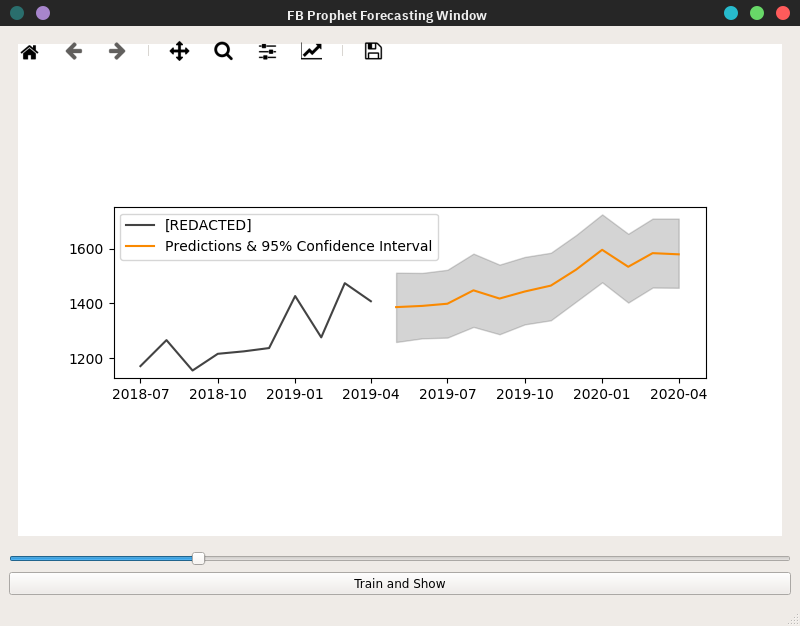
\includegraphics[width=0.5\textwidth]{Images/slider-1.png}   % Just a dummy. Replace with your figure.
      }
      \ffigbox[\FBwidth]{\caption{Slider at a position on the right-hand side}\label{fig:dummy-2}}{%
        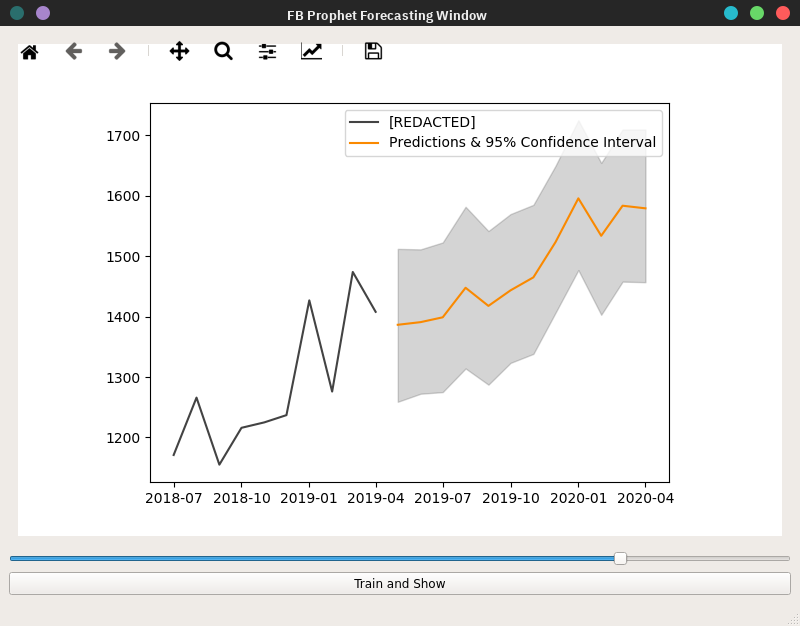
\includegraphics[width=0.5\textwidth]{Images/slider-2.png}   % Just a dummy. Replace with your figure.
      }
    \end{floatrow}
  \end{figure}
\end{center}
\subsection{Testing Phase}
\label{sec:testing}
The software was mainly tested by hand. The problems discussed in Section \ref{sec:prophet-issues} were the most time consuming, and issues with Matplotlib components (see section \ref{sec:matplotlib-issues}) were resolved with a GUI slider. \\
On the accuracy of the forecast, we've seen MAPE (Mean Absolute Percentage Errors) while training as in the range of $1\%$ to $2\%$, but some types of data proved to be extremely difficult to forecast, receiving errors of about $7\%$. As a computer engineering student with no economics background, these results seemed to be an outlier in the tests, and were left to be fixed by the data science team at the company. \\
Further tests on the accuracy of predictions were presumably done by the company, but as of time of this report, these tests were not disclosed with us.
\section{About JotForm Inc.}
JotForm is an international company, having offices in San Francisco, Izmir, and Ankara. Managerial
staff is primarily located in Ankara office, which is also the home for the main R\&D hub for the company. \\
\begin{figure}[hbt!]
    \centering
    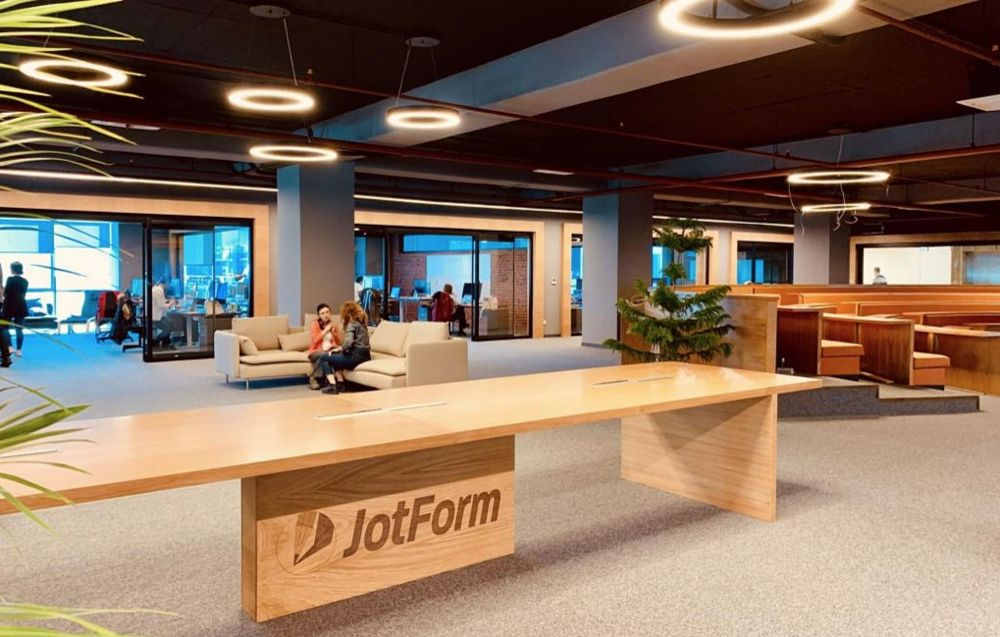
\includegraphics[width=0.9\textwidth]{Images/new-turkey-office.jpg}
    \caption{A View From JotForm's Ankara Offices}
    \label{fig:JFMAnkara}
\end{figure} \\
\subsection{Structure of the company}
In JotForm, employees are operating in teams, named by themselves, such as Amplify, Hermes and so on. The main responsibility of a team is not divided between different products of the company. This way, they can keep their focus, and work more reliably as a team. A team, for example, may work on Form Builder for a certain amount of time, and not in other products such as PDF Editor. This allows for an efficitent \textbf{Agile} work environment. \\
On fridays, all teams from Izmir and Ankara offices of JotForm come together for a meet, called the Demo Day. This facilitates for the presentations of the work done in the week for each team. This day is also the day for us interns to perform their presentations about their projects.

\subsection{Products offered by JotForm}
\subsubsection{Form Builder}
Form Builder tool is the main product of the company. Offering a drag-and-drop interface for creating forms,
analyzing data easily and making the analysis of the results from the form easier (using JotForm Sheets) is the main focus of the company. Since 2006, the founding of the company, they operate a Form Builder interface, which is active to this day. Main differences from competitors such as Google Sheets is the ease of use, and options for payment such as PayPal, Stripe etc. , which makes the product a standalone candidate for e-commerce websites, handling payments and billing information all by itself.

\subsubsection{PDF Editor}
In the last year, JotForm offices in Ankara started a project on PDF documents. Since the main focus of the company is on the forms, and customers repeatedly reporting that they need to convert their PDF forms to some online form, a team in Ankara office has built a tool for the purpose. In PDF editor, users can upload their fill-able PDF forms, and automatically transform them into an online form, hosted on JotForm. This feature also works in the other way around, as in, a user can take an existing online form in JotForm, and turn it into a fill-able PDF file format.

\subsubsection{JotForm Sheets}
Primarily to relieve their customers from needing to resort to Google's services, mainly, Google Sheets, the company developed a tool to deal with Spreadsheet files.
This is integrated into their form builder environment, so that the customers can perform aggregate functions similar to Microsoft Excel™, analyze large amount of responses to their forms, and export to useful file formats, such as .csv files. 
%\section{Methodology}
%% Methodology or Algorithm or Theoretical know-how or steps to run your code/simulations
% Please delete the below lines and enter details for this assignment/homework

    This section should be dedicated to explaining the 'theoretical know-how' or 'steps to run your code' or 'algorithms used'. 

The following are guidelines. Use your judgment appropriately

\begin{enumerate}
\item Explain your approach to solving this homework assignment (theoretical know-how)
\item Which concepts from the class did you apply in this homework?  How did you apply them? State the assumptions made, including the reason for assumptions.
\item Are there any special steps that should be followed to run/simulate your program/files on other computer, with necessary software (MATLAB/MULTISIM)?
\item Explain the main parts of your algorithm with the help of a flowchart, if appropriate. What does each section of it do? 
\end{enumerate}




 Note:
\begin{itemize}
\item  In MATLAB, Lines of comment embedded in the program are essential. However, comments cannot be used as a substitute for the algorithm explanations asked for above!
\item  Remember, these questions are just examples to guide you in explaining your methodology. You may not need to answer all of them in all homework assignments. You may need to add more information in a particular report. Use your judgment appropriately!
\end{itemize}




%\section{Results}
%% Results
% Please delete the below lines and enter details for this assignment/homework
\begin{itemize}
\item  The results obtained should be placed here. Attach the screen shots (with description labels) from your simulation to show the schematic circuit, static/transient response, other results, as per the homework/assignment. Also, if something unexpected happened (errors/issues), attach screen shot (with description labels). Use graphs when appropriate to demonstrate results. 
\end{itemize}

%\section{Discussions and Conclusion}
%% Discussions & Conclusion
% Please delete the below lines and enter details for this assignment/homework
    Finally, discuss your results and state your conclusions on the task you were given in this
homework.
\begin{enumerate}
\item Did you meet the goals of this homework?
\item What was the key elements of theoretical know-how taken into consideration ?
\item If there is any errors/issues, what do you think about this error/issue? How can you do to fix it?
\item If your simulation/calculation works mostly as expected, but fails in some scenarios, what do you think or state the possible reasons, try to propose a solution?
\item What are the limitations of your code/simulation?
\item Make a comment about how this homework affected your knowledge of the subject.
\end{enumerate}


\bibliographystyle{plainurl}
\bibliography{Bibliography.bib}

%\appendix
%\section{Appendix}
%%
% Please attach the MATLAB or MULTISIM files (finial version) with this report
% Please delete the below lines and enter details for this assignment/homework
 Include your code here! \\
 
\textbf{ Note: Also ensure to attach the MATLAB or MULTISIM files with this report.}



%---------------------------------------------------------------------------------
%	Example SECTION (Remove this section to finalize the report.


%\section{Example steps}
%% These are some example steps 
% Refer https://www.overleaf.com/learn/how-to/Creating_a_document_in_Overleaf


\subsection{Sub Sections}

Use section and subsection commands to organize your document. \LaTeX{} handles all the formatting and numbering automatically. Use ref and label commands for cross-references.

\subsection{Comments}

Comments can be added to the margins of the document using the \todo{Here's a comment in the margin!} todo command, as shown in the example on the right. You can also add inline comments too:

\todo[inline, color=green!40]{This is an inline comment.}

\subsection{Tables and Figures}

Use the table and tabular commands for basic tables --- see Table~ \ref{tab:widgets}, for example. You can upload a figure (JPEG, PNG or PDF) using the files menu. To include it in your document, use the include graphics command as in the code for Figure~\ref{fig:Speed vs. Torque from Pittman} below.

\begin{table}[h]
\centering
\begin{tabular}{|l|r|}
\hline
Item & Quantity \\\hline
Widgets & 42 \\ \hline
Gadgets & 13 \\ \hline
\end{tabular}
\caption{\label{tab:widgets}An example table.}
\end{table}

% Commands to include a figure:
\begin{figure}[hbt!]
    \centering
    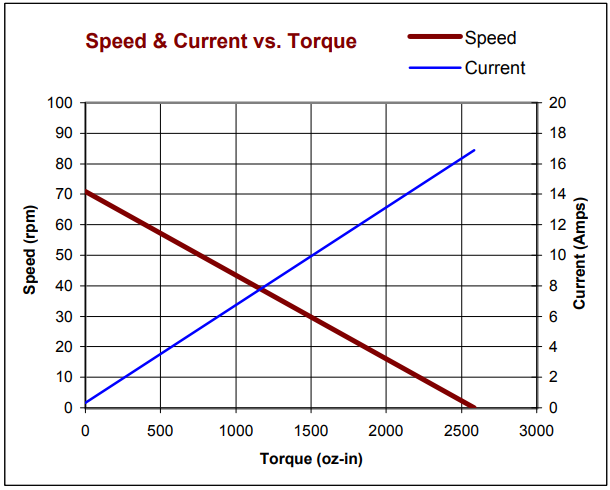
\includegraphics[width=0.9\textwidth]{Images/SpeedvsTorque.png}
    \caption{Speed vs. Torque from Pittman motor data sheet}
    \label{fig:Speed vs. Torque from Pittman}
\end{figure}





\subsection{Mathematics}

\LaTeX{} is great at typesetting mathematics. Let $X_1, X_2, \ldots, X_n$ be a sequence of independent and identically distributed random variables with $\text{E}[X_i] = \mu$ and $\text{Var}[X_i] = \sigma^2 < \infty$, and let
$$S_n = \frac{X_1 + X_2 + \cdots + X_n}{n}
      = \frac{1}{n}\sum_{i}^{n} X_i$$
denote their mean. Then as $n$ approaches infinity, the random variables $\sqrt{n}(S_n - \mu)$ converge in distribution to a normal $\mathcal{N}(0, \sigma^2)$.

\subsection{Lists}

You can make lists with automatic numbering \dots

\begin{enumerate}
\item Like this,
\item and like this.
\end{enumerate}
\dots or bullet points \dots
\begin{itemize}
\item Like this,
\item and like this.
\end{itemize}

%% cite an article
\subsection{Bibliography}
\begin{itemize}
    \item Adding bibliography to document
	\item Some claim \cite{gratzer2007more}.
\end{itemize}

\subsection{Hyperlink to a website}
%% Hyperlink to a website
\begin{itemize}
    \item \href{https://www.overleaf.com/latex/templates/a-quick-guide-to-latex/fghqpfgnxggz}{Hyperlink to a website}.
\end{itemize}



\subsection{Learn LaTeX in 30 minutes}
\begin{itemize}
    \item \href{https://www.overleaf.com/learn/latex/Learn_LaTeX_in_30_minutes}{Link to overleaf website}.
\end{itemize}

 % Remove this line to finalize the report.
%---------------------------------------------------------------------------------


\end{document}


% Note: Again, you don’t need to answer just the above questions. They are being provided to give you a flavor of what is required for each section. Use your judgment and initiative to add or subtract based on the specific homework. You can add any other conclusion or discuss any other aspect of your effort that you think it is important to highlight.

% Also ensure to attach the MATLAB or MULTISIM files with this report